\documentclass[12pt,a4paper,oneside]{report}
\usepackage[utf8]{inputenc}
\usepackage[english]{babel}
\usepackage{geometry}
\geometry{left=3cm,right=2cm,top=2.5cm,bottom=2.5cm}
\usepackage{amsmath}
\usepackage{amssymb}
\usepackage{booktabs}
\usepackage{graphicx}
\usepackage{listings}
\usepackage{color}
\usepackage{setspace}
\usepackage{hyperref}
\usepackage{tikz}
\usepackage{float}
\usepackage{multirow}
\usepackage{enumitem}
\usepackage[acronym,toc]{glossaries}
\usepackage{algorithm}
\usepackage{algpseudocode}
\usetikzlibrary{shapes.geometric, arrows.meta, positioning, fit, backgrounds, calc}

% Algorithm translations
\floatname{algorithm}{Algorithm}
\renewcommand{\listalgorithmname}{List of Algorithms}
\renewcommand{\lstlistingname}{Listing}

\hypersetup{
    colorlinks=true,
    linkcolor=blue,
    citecolor=blue,
    filecolor=magenta,
    urlcolor=cyan,
    pdftitle={Thesis Report - Hybrid RAG},
}

% 1.5 line spacing
\onehalfspacing

% Definition of colors for code blocks
\definecolor{codegreen}{rgb}{0,0.6,0}
\definecolor{codegray}{rgb}{0.5,0.5,0.5}
\definecolor{codepurple}{rgb}{0.58,0,0.82}
\definecolor{backcolour}{rgb}{0.95,0.95,0.92}

\lstdefinestyle{mystyle}{
    backgroundcolor=\color{backcolour},
    commentstyle=\color{codegreen},
    keywordstyle=\color{magenta},
    numberstyle=\tiny\color{codegray},
    stringstyle=\color{codepurple},
    basicstyle=\ttfamily\footnotesize,
    breakatwhitespace=false,
    breaklines=true,
    captionpos=b,
    keepspaces=true,
    numbers=left,
    numbersep=5pt,
    showspaces=false,
    showstringspaces=false,
    showtabs=false,
    tabsize=2
}
\lstset{style=mystyle}

% TikZ styles for architecture diagrams
\tikzset{
    component/.style={rectangle, draw=black!60, fill=blue!8, thick, minimum height=1cm, minimum width=3.5cm, text centered, font=\small},
    storage/.style={cylinder, draw=black!60, fill=purple!8, thick, minimum height=1cm, minimum width=2.5cm, text centered, font=\small, shape border rotate=90, aspect=0.25},
    process/.style={rectangle, rounded corners, draw=black!60, fill=green!8, thick, minimum height=0.8cm, minimum width=3cm, text centered, font=\small},
    arrow/.style={-{Stealth[length=3mm]}, thick},
    dasharrow/.style={-{Stealth[length=3mm]}, thick, dashed},
    groupbox/.style={rectangle, rounded corners, draw=black!40, dashed, inner sep=0.4cm},
}

% ──────────────────────────────────────────────────────────────────────────────
% GLOSSARY / ABBREVIATIONS
% ──────────────────────────────────────────────────────────────────────────────
\newacronym{rag}{RAG}{Retrieval-Augmented Generation}
\newacronym{llm}{LLM}{Large Language Model}
\newacronym{ast}{AST}{Abstract Syntax Tree}
\newacronym{rrf}{RRF}{Reciprocal Rank Fusion}
\newacronym{fqn}{FQN}{Fully Qualified Name}
\newacronym{kg}{KG}{Knowledge Graph}
\newacronym{sla}{SLA}{Service Level Agreement}
\newacronym{dod}{DOD}{Definition of Done}
\newacronym{api}{API}{Application Programming Interface}
\newacronym{mrr}{MRR}{Mean Reciprocal Rank}
\newacronym{mro}{MRO}{Method Resolution Order}
\newacronym{mcp}{MCP}{Model Context Protocol}
\newacronym{ui}{UI}{User Interface}

\makeglossaries

\begin{document}

% ──────────────────────────────────────────────────────────────────────────────
% COVER PAGE
% ──────────────────────────────────────────────────────────────────────────────
\begin{titlepage}
    \begin{center}
        \large MINISTRY OF EDUCATION AND TRAINING \\
        \textbf{\large FPT UNIVERSITY} \\
        \vfill
        \textbf{\Large MASTER'S THESIS} \\
        \vfill
        \begin{singlespace}
            \textbf{\Large RESEARCH AND DEVELOPMENT OF A CODE RETRIEVAL SYSTEM BASED ON HYBRID-RAG ARCHITECTURE COMBINING KNOWLEDGE GRAPHS AND SEMANTIC SEARCH}
        \end{singlespace}
        \vfill
        \vspace{1.5cm}
        \begin{tabular}{rll}
            Student: & Tran Tien Duat \\
            Student ID: & XXXXXXXX \\
            Degree: & Master of Software Engineering \\
            Advisor: & Doan Xuan Huy Minh \\
        \end{tabular}
        \vfill
        \large HO CHI MINH CITY, YEAR 2026
    \end{center}
\end{titlepage}

\tableofcontents
\newpage
\listoffigures
\newpage
\listoftables
\newpage
\printglossary[type=\acronymtype, title=List of Abbreviations]
\newpage

% ──────────────────────────────────────────────────────────────────────────────
% ABSTRACT
% ──────────────────────────────────────────────────────────────────────────────
\chapter*{Abstract}
\addcontentsline{toc}{chapter}{Abstract}
Code querying is a complex problem because source code contains both static structural information (function calls, class inheritance, and module definitions) and semantic information. A vector-only \gls{rag} index can represent semantic similarity, but it does not directly expose typed code relations for relation-heavy questions.

This thesis designs and evaluates a \textbf{Hybrid-RAG} architecture that combines an \gls{ast}-derived \gls{kg} in FalkorDB with dense retrieval in Qdrant. The implementation uses query-aware graph traversal, vector search, weighted \gls{rrf} \cite{cormack2009rrf}, and token-budgeted context assembly. A paired benchmark on 30 reviewed questions from one pinned LlamaIndex Core snapshot produced 180 generated and scored answers. Hybrid-RAG obtained mean Faithfulness 0.924, Answer Relevancy 0.808, and Answer Correctness 0.698, versus 0.896, 0.729, and 0.652 for vector-only retrieval. Paired case-level 95\% bootstrap intervals for the Hybrid-minus-vector differences were $[-0.069, 0.115]$, $[-0.0001, 0.175]$, and $[0.002, 0.094]$, respectively. Thus, only the observed Answer Correctness difference excludes zero at the 95\% level. All embedding, generation, and judging calls used local Ollama services. The evidence is limited to one Python repository and one executed baseline; it does not establish cross-repository or cross-language generality.

\newpage

% ──────────────────────────────────────────────────────────────────────────────
% CHAPTER 1: INTRODUCTION
% ──────────────────────────────────────────────────────────────────────────────
\chapter{Introduction}

\section{System Context}
Modern software maintenance requires developers to navigate large, evolving codebases and recover relationships that are distributed across files and modules. \glspl{llm} create new opportunities for programming assistance \cite{chen2021codex}; however, placing an entire repository in one prompt is constrained by finite context budgets and by degraded use of information located in the middle of long contexts \cite{liu2023lost}.

The \gls{rag} technique \cite{lewis2020rag} addresses this problem by retrieving a bounded set of source evidence and inserting it into the \gls{llm} context. A vector-only implementation can retrieve semantically related code, but its index does not explicitly represent call, import, definition, or inheritance edges. This motivates testing whether an AST-derived graph channel adds useful evidence beyond the same system operated in vector-only mode.

\section{Problem Statement and Bottlenecks}
The research problem is to retrieve evidence for questions that combine semantic intent with repository-specific structure while keeping the source and model calls local. Four gaps shape the work:

\begin{itemize}
    \item \textbf{Representation gap:} dense chunks encode semantic similarity but not explicit repository topology.
    \item \textbf{Context constraint:} source evidence must be selected and serialized within a bounded prompt budget.
    \item \textbf{Index integrity:} repository identity, source revision, schema, and embedding model must remain consistent across graph and vector stores.
    \item \textbf{Evidence gap:} positive point estimates from one repository are insufficient for broad claims without paired uncertainty estimates, additional repositories, and stronger baselines.
\end{itemize}

\section{Related Works}
To solve the code querying problem, existing technologies exhibit various strengths and limitations. Table~\ref{tab:related_works} presents a comparison matrix of the solutions:

\begin{table}[H]
    \centering
    \caption{Comparison matrix of current code querying solutions}
    \label{tab:related_works}
    \small
    \begin{tabular}{p{2.5cm}p{3cm}p{3cm}p{4.5cm}}
        \toprule
        \textbf{Solution} & \textbf{Core Mechanism} & \textbf{Role in this thesis} & \textbf{Main trade-off} \\
        \midrule
        \textbf{BM25 / lexical retrieval} \cite{bm25} & Exact-term ranking & Literature baseline; not executed & Strong symbol matching / weak paraphrase handling. \\
        \midrule
        \textbf{Vector-only RAG} \cite{lewis2020rag} & Dense chunks + cosine similarity & Executed baseline & Semantic matching / no explicit topology. \\
        \midrule
        \textbf{Code encoders} (CodeBERT \cite{feng2020codebert}, GraphCodeBERT \cite{guo2024graphcodebert}) & Pre-trained code representation & Literature comparison; not executed & Learned code semantics / requires model-specific indexing. \\
        \midrule
        \textbf{Microsoft GraphRAG} \cite{edge2024graphrag} & Entity graph + community summaries & Architectural comparison; not executed & Global synthesis / additional indexing and summarization work. \\
        \midrule
        \textbf{This prototype} & AST graph + dense retrieval + weighted \gls{rrf} & Evaluated against vector-only & Structural and semantic evidence / higher retrieval latency and indexing complexity. \\
        \bottomrule
    \end{tabular}
\end{table}

The comparison separates related approaches from executed baselines. Only vector-only retrieval is run under the same source snapshot, models, questions, and repeated-measure protocol. BM25, graph-only retrieval, code encoders, and Microsoft GraphRAG remain necessary baselines for a broader comparative study.

\section{Proposed Solution}
We propose a query-aware Hybrid-RAG solution using FalkorDB \cite{falkordb2024} and Qdrant \cite{qdrant2024}. Exact relation questions use deterministic graph traversal when a relation target is found; other local questions can search graph and vector channels concurrently and fuse their rankings with weighted \gls{rrf}; global questions retrieve repository-scoped community summaries. The selected evidence is assembled under a token or character budget before local generation. Chapter 2 derives this design from the literature, and Chapter 3 maps it to the implementation.

\section{Research Gap and Technical Contributions}
Hybrid retrieval, AST parsing, graph retrieval, and RRF are established techniques. The thesis therefore does not claim a new retrieval algorithm. Its contribution is an evidence-backed system design and integration for private codebase understanding:
\begin{itemize}
    \item a repository-scoped dual index that maps Python AST entities and typed relations to FalkorDB while storing source-aligned semantic chunks in Qdrant;
    \item query-aware retrieval that combines deterministic relation traversal, concurrent graph--vector retrieval, weighted rank fusion, sibling expansion, and budgeted context assembly;
    \item integrity controls including conservative entity resolution, replacement-before-delete index updates, source/schema/model provenance validation, cache-generation invalidation, and a local-only Ollama boundary; and
    \item a reproducible paired answer-quality benchmark with raw records and case-level confidence intervals, together with explicit limits on repository, language, and baseline coverage.
\end{itemize}

\section{Research Objectives \& Questions}

\subsection{Research Objectives}
The primary objective is to determine whether adding AST-derived structural retrieval to an otherwise identical vector-RAG pipeline improves grounded answers about a Python codebase under local execution constraints. The specific objectives are:
\begin{itemize}
    \item implement a repository-scoped graph--vector retrieval pipeline with reproducible source provenance and bounded context assembly;
    \item compare Hybrid-RAG with vector-only retrieval using the same questions, source snapshot, models, and repeated runs; and
    \item quantify answer quality, retrieval/generation latency, and token usage with paired confidence intervals while documenting threats to validity.
\end{itemize}

\subsection{Research Questions}
The thesis addresses three research questions aligned with the available measurements:
\begin{itemize}
    \item \textbf{RQ1 --- Answer quality:} Under the pinned LlamaIndex workload, how does Hybrid-RAG change Faithfulness, Answer Relevancy, and Answer Correctness relative to vector-only retrieval?
    \item \textbf{RQ2 --- Efficiency trade-off:} What changes in retrieval latency, local generation latency, and prompt/completion token counts accompany Hybrid-RAG?
    \item \textbf{RQ3 --- Evidence strength:} Which observed differences remain above or below zero under paired case-level 95\% confidence intervals, and what limits their generalization?
\end{itemize}

\section{Research Scope \& Definition of Done}
\subsection{Research Scope}
The evaluated implementation is scoped to Python. Java indexing is explicitly rejected because a Java entity extractor and resolver are not implemented, even though a Java grammar is used by the separate context skeletonizer. The completed answer-quality benchmark covers one pinned repository (\texttt{llama-index-core==0.14.21}) and one executed baseline (vector-only). It uses \texttt{nomic-embed-text} for embeddings, \texttt{gemma4:12b} for answer generation, and \texttt{qwen2.5-coder:7b} as an independent local judge. Results for Transformers, LangChain, Kubernetes, BM25, graph-only retrieval, or Microsoft GraphRAG are not available and are not inferred.

\subsection{Definition of Done (DoD)}
The evaluated prototype uses the following evidence criteria:
\begin{enumerate}
    \item persist complete raw records for both retrieval modes under a pinned source identity and index schema;
    \item report Faithfulness, Answer Relevancy, and Answer Correctness with paired case-level 95\% confidence intervals;
    \item report retrieval latency separately from local generation latency and token counts; and
    \item treat cross-repository, cross-language, and additional-baseline conclusions as unverified until dedicated experiments are completed.
\end{enumerate}

\newpage

% ──────────────────────────────────────────────────────────────────────────────
% CHAPTER 2: SYSTEM ARCHITECTURE
% ──────────────────────────────────────────────────────────────────────────────
\chapter{Theoretical Background and System Architecture}

\section{Theoretical Background \& Literature Review}

\subsection{Information Retrieval (IR) Theory}
Information Retrieval (IR) is the process of obtaining information resources relevant to an information need from a collection of resources. In modern search pipelines, two primary IR paradigms dominate:
\begin{itemize}
    \item \textbf{Lexical Retrieval (Keyword Matching):} Classical retrieval algorithms like TF-IDF and BM25 \cite{bm25} match query terms against document terms. The BM25 score of a document $D$ for a query $Q$ with terms $q_i$ is computed as:
    \begin{equation}
        \text{Score}(D, Q) = \sum_{i=1}^{n} \text{IDF}(q_i) \cdot \frac{f(q_i, D) \cdot (k_1 + 1)}{f(q_i, D) + k_1 \cdot \left(1 - b + b \cdot \frac{|D|}{\text{avgdl}}\right)}
    \end{equation}
    where $f(q_i, D)$ is the term frequency in the document, $|D|$ is the document length, and $\text{avgdl}$ is the average document length. BM25 is highly effective at finding exact class names, method signatures, or variables in codebases. However, it fails when queries use synonyms or semantic descriptions that do not match exact characters.
    
    \item \textbf{Dense Semantic Retrieval:} Dense retrieval utilizes neural embedding models to convert text into high-dimensional vector spaces. Semantic similarity between query vector $\mathbf{u}$ and document vector $\mathbf{v}$ is computed using Cosine Similarity:
    \begin{equation}
        \text{Similarity}(\mathbf{u}, \mathbf{v}) = \frac{\mathbf{u} \cdot \mathbf{v}}{\|\mathbf{u}\| \|\mathbf{v}\|}
    \end{equation}
    While dense retrieval captures abstract user intent, it is susceptible to noise and ignores the strict lexical syntax and structural morphology unique to software codebases.
\end{itemize}

\subsection{Code Search Models}
Source code fundamentally differs from natural language due to its strict structural syntax and logic constraints. Code representation models have evolved through three generations:
\begin{enumerate}
    \item \textbf{Text-based Representation:} Treating code as plain text, utilizing BM25 or regex searches. This completely discards programming grammar.
    \item \textbf{Deep Pre-trained Language Models:} Models such as CodeBERT \cite{feng2020codebert} and GraphCodeBERT \cite{guo2024graphcodebert} learn code representations from large corpora; GraphCodeBERT additionally incorporates data-flow structure. They operate on bounded inputs and do not by themselves maintain an explicit, updateable graph of repository-specific relationships.
    \item \textbf{Static Dependency Graphs:} Leveraging language parsers to build static relationship maps. Formally, we define the codebase knowledge graph as a directed multigraph $G = (V, E, \phi, \psi)$, where:
    \begin{itemize}
        \item $V$ is the set of emitted AST code entity nodes (Module, Class, Function).
        \item $E$ is the set of directed edges representing syntax relations.
        \item $\phi: V \rightarrow L_V$ is the node labeling function mapping vertices to $L_V = \{\text{Module}, \text{Class}, \text{Function}\}$.
        \item $\psi: E \rightarrow L_E$ is the edge labeling function mapping connections to syntax dependencies $L_E = \{\text{DEFINES}, \text{CALLS}, \text{INHERITS}, \text{IMPORTS}\}$.
    \end{itemize}
\end{enumerate}

\subsection{Retrieval-Augmented Generation (RAG) and Graph RAG}
Retrieval-Augmented Generation (RAG) \cite{lewis2020rag} optimizes LLM performance by injecting external context into the prompt. The paradigm has evolved as follows:
\begin{itemize}
    \item \textbf{Naive RAG:} Chunks source code at fixed text boundaries. Such windows can split functions or classes and lose structural context.
    \item \textbf{Advanced RAG:} Introduces syntax-aware chunking based on AST boundaries (Class/Function scopes) and post-retrieval reranking.
    \item \textbf{Graph RAG:} Incorporates a knowledge-graph index. Frameworks such as Microsoft GraphRAG \cite{edge2024graphrag} use entity extraction and hierarchical community summaries for global questions. This adds an indexing and summarization stage whose quality, latency, and compute cost depend on the selected models and corpus.
\end{itemize}
To combine the benefits of both dense semantic and structural retrieval, we propose a Hybrid-RAG system coordinated via Reciprocal Rank Fusion (RRF) \cite{cormack2009rrf}:
\begin{equation}
    RRF\_Score(d \in D) = \sum_{m \in M} \frac{w_m}{k + r_m(d)}
\end{equation}
where $M = \{\text{vector}, \text{graph}\}$, $r_m(d)$ is the rank of document $d$ in retrieval stream $m$, $w_m$ is the weight of the retrieval stream, and $k$ is a smoothing parameter set to 60 in this implementation. Rank fusion avoids assuming that vector similarities and graph scores share a calibrated numerical scale.

\subsection{Literature Synthesis and Design Implications}
The reviewed approaches are complementary rather than interchangeable. Lexical retrieval is useful for exact identifiers; dense retrieval covers paraphrased intent; AST and dependency graphs expose typed relations; and RAG constrains generation to selected evidence. This synthesis leads to five design decisions: (i) parse code at symbol boundaries instead of fixed character windows, (ii) store semantic chunks and typed graph relations in separate indexes, (iii) route explicit relation questions to deterministic graph plans, (iv) use rank fusion when both channels contribute candidates, and (v) assemble the final evidence under a strict context budget with source metadata. The implementation evaluates the incremental value of the graph channel against vector-only retrieval. It does not evaluate every approach in the literature, so BM25, graph-only, learned code encoders, and Microsoft GraphRAG remain comparison gaps rather than measured inferiors.

\section{System Architecture}

\section{System Requirements}
\begin{itemize}
    \item \textbf{Functional Requirements:} The system must support static source code parsing to construct relationship graphs, semantic search based on cosine similarity, hybrid querying (combining graph structures and text), and return answers alongside precise code references.
    \item \textbf{Non-functional Requirements (\gls{sla}):} Retrieval response latency $< 1s$ as a retrieval target, concurrency support during embedding generation, and a local-only model-provider boundary.
\end{itemize}

\section{High-level Architecture}
The Hybrid-RAG system is designed following the Hexagonal architecture (Ports and Adapters) \cite{cockburn2005hexagonal} to decouple physical database infrastructure layers from the core search engine business logic. The overall architecture and data flow are described in Figure~\ref{fig:architecture_overview}.

\begin{figure}[H]
    \centering
    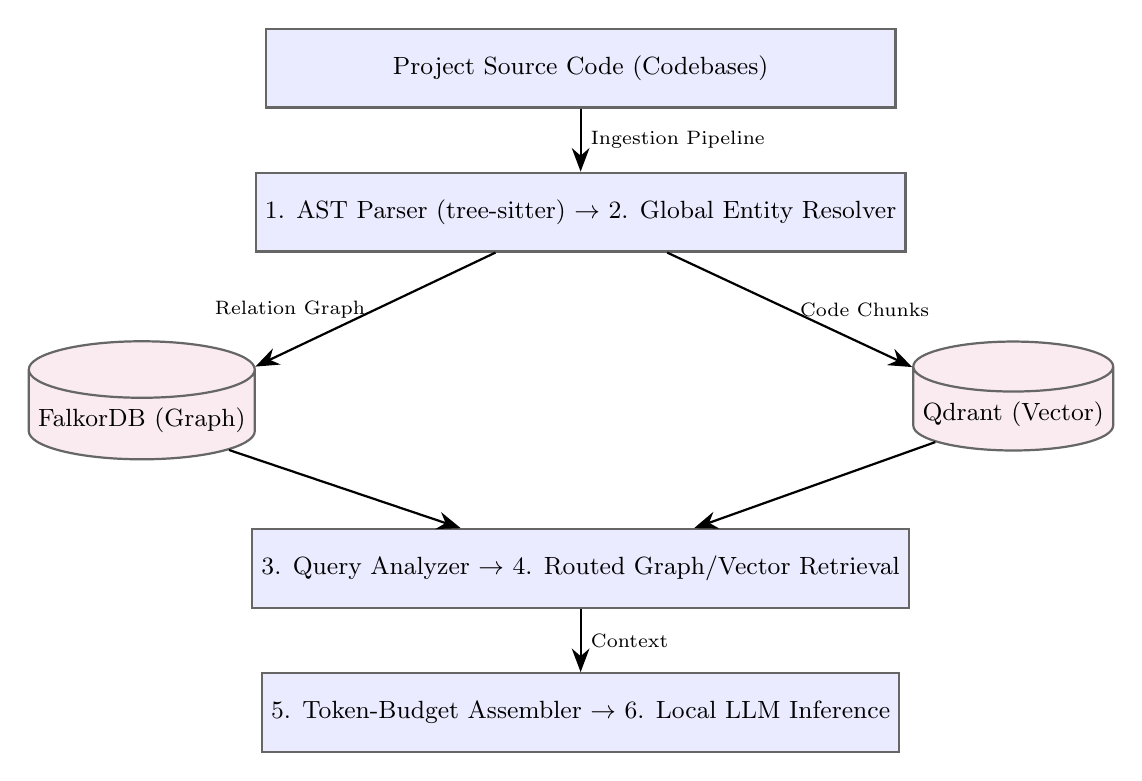
\begin{tikzpicture}[node distance=0.8cm and 1.5cm, font=\small]
        % Ingestion Pipeline
        \node[component, minimum width=8cm] (codebase) {Project Source Code (Codebases)};
        \node[component, minimum width=8cm, below=of codebase] (ingestion) {1. AST Parser (tree-sitter) $\to$ 2. Global Entity Resolver};

        % Storage
        \node[storage, below left=1.2cm and 0.5cm of ingestion] (falkor) {FalkorDB (Graph)};
        \node[storage, below right=1.2cm and 0.5cm of ingestion] (qdrant) {Qdrant (Vector)};

        % Retrieval
        \node[component, minimum width=8cm, below=3.5cm of ingestion] (retrieval) {3. Query Analyzer $\to$ 4. Routed Graph/Vector Retrieval};

        % Inference
        \node[component, minimum width=8cm, below=of retrieval] (inference) {5. Token-Budget Assembler $\to$ 6. Local LLM Inference};

        % Arrows
        \draw[arrow] (codebase) -- node[right, font=\scriptsize] {Ingestion Pipeline} (ingestion);
        \draw[arrow] (ingestion) -- node[left, font=\scriptsize] {Relation Graph} (falkor);
        \draw[arrow] (ingestion) -- node[right, font=\scriptsize] {Code Chunks} (qdrant);
        \draw[arrow] (falkor) -- (retrieval);
        \draw[arrow] (qdrant) -- (retrieval);
        \draw[arrow] (retrieval) -- node[right, font=\scriptsize] {Context} (inference);
    \end{tikzpicture}
    \caption{Overall data flow diagram of the Hybrid-RAG system}
    \label{fig:architecture_overview}
\end{figure}

\section{Ingestion Pipeline}
The ingestion pipeline converts raw source code into structural relationship graphs and semantic embedding vectors. This process consists of 4 main phases, as illustrated in Figure~\ref{fig:ingestion_sequence}:

\begin{enumerate}
    \item \textbf{Phase 1 --- AST Parsing:} The Tree-Sitter library \cite{treesitter} parses Python source code into Abstract Syntax Trees. The system extracts entities (Module, Class, Function) and automatically assigns dot-notated \gls{fqn} strings (\texttt{package.module.Class.method}) to ensure uniqueness across the repository. Java projects are rejected at the indexing boundary until a Java extractor is implemented.
    \item \textbf{Phase 2 --- Global Entity Resolution:} Unresolved call stubs are resolved conservatively using caller context: (i) methods in the same class, (ii) module-level functions in the caller's module, and (iii) import-aware unique candidates. Remaining stubs are matched in one batch against previously indexed graph nodes and redirected only when exactly one target exists. The algorithm details are described in Section~\ref{sec:entity_resolution}.
    \item \textbf{Phase 3 --- Source Code Chunking:} Source code is chunked at AST function and class boundaries instead of fixed character windows, preserving symbol-level boundaries where parsing succeeds.
    \item \textbf{Phase 4 --- Parallel Embedding:} Chunks are embedded through a bounded \texttt{ThreadPoolExecutor}; the default \texttt{EMBED\_CONCURRENCY} is 8. The \texttt{nomic-embed-text} model \cite{nussbaum2024nomic} generates 768-dimensional vectors through local Ollama \cite{ollama2024}. No controlled sequential-versus-parallel embedding benchmark is reported in this thesis.
\end{enumerate}

\begin{figure}[H]
    \centering
    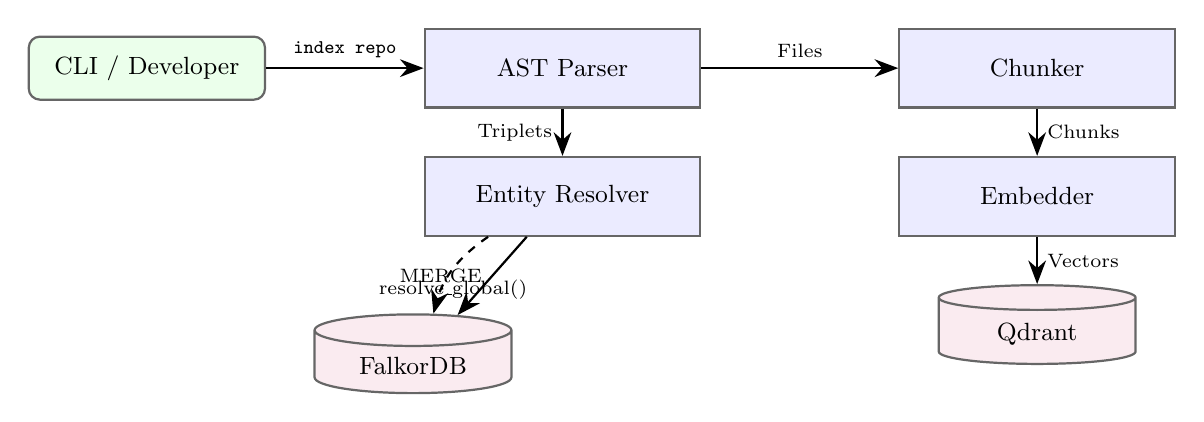
\begin{tikzpicture}[node distance=0.6cm and 0.8cm, font=\small]
        % Nodes
        \node[process] (cli) {CLI / Developer};
        \node[component, right=2cm of cli] (parser) {AST Parser};
        \node[component, below=of parser] (resolver) {Entity Resolver};
        \node[storage, below left=1cm and -0.5cm of resolver] (fdb) {FalkorDB};
        \node[component, right=2.5cm of parser] (chunker) {Chunker};
        \node[component, below=of chunker] (embedder) {Embedder};
        \node[storage, below=of embedder] (qdr) {Qdrant};

        % Arrows
        \draw[arrow] (cli) -- node[above, font=\scriptsize] {\texttt{index repo}} (parser);
        \draw[arrow] (parser) -- node[left, font=\scriptsize] {Triplets} (resolver);
        \draw[arrow] (resolver) -- node[left, font=\scriptsize] {MERGE} (fdb);
        \draw[arrow] (parser) -- node[above, font=\scriptsize] {Files} (chunker);
        \draw[arrow] (chunker) -- node[right, font=\scriptsize] {Chunks} (embedder);
        \draw[arrow] (embedder) -- node[right, font=\scriptsize] {Vectors} (qdr);
        \draw[dasharrow] (resolver) to[bend right=20] node[below, font=\scriptsize] {resolve\_global()} (fdb);
    \end{tikzpicture}
    \caption{Data processing flow of the Ingestion Pipeline}
    \label{fig:ingestion_sequence}
\end{figure}

\subsection{Incremental Indexing and Synchronization}
To prevent parsing and embedding the entire repository from scratch upon every codebase change (which is CPU/GPU and time intensive), the system implements an incremental indexing and synchronization mechanism:
\begin{itemize}
    \item \textbf{Commit Hash Tracking:} The system persists the last indexed commit hash for each repository directly inside the FalkorDB graph database.
    \item \textbf{Change Detection:} During re-indexing, the system leverages Git diff mappings to isolate modified, added, renamed, or deleted files.
    \item \textbf{Targeted Cleanup:} Before processing new changes, the system executes targeted queries to purge the old AST entities of modified/deleted files from FalkorDB and deletes their corresponding vector points from Qdrant.
    \item \textbf{Delta Processing:} Only newly added or modified files are passed through the ingestion pipeline. The implementation reduces repeated work by construction, but this thesis does not report a controlled percentage reduction for incremental indexing.
\end{itemize}

\subsection{Monorepo and Subdirectory Support}
To meet modern industrial software engineering requirements, the ingestion pipeline implements a recursive upward Git repository resolution algorithm. In multi-package monorepos, codebase paths defined in the configurations often target specific nested package subdirectories rather than the root directory. By recursively traversing the file tree upwards from the configured subdirectory path until it detects a valid \texttt{.git} folder, the system correctly identifies and resolves the monorepo root. This ensures that change detection, commit tracking, and incremental diff synchronization function correctly and transparently across individual monorepo components without requiring independent Git setups.

\section{Hybrid Retrieval Flow}
The query analyzer selects among three implemented paths. Global questions return repository-filtered community summaries. Explicit relation questions first execute a deterministic graph plan and fall back to vector retrieval only when no relation target is found. Generic local questions search the graph and vector channels concurrently and fuse their ranks. Figure~\ref{fig:retrieval_flow} shows this third, generic-local path:

\begin{figure}[H]
    \centering
    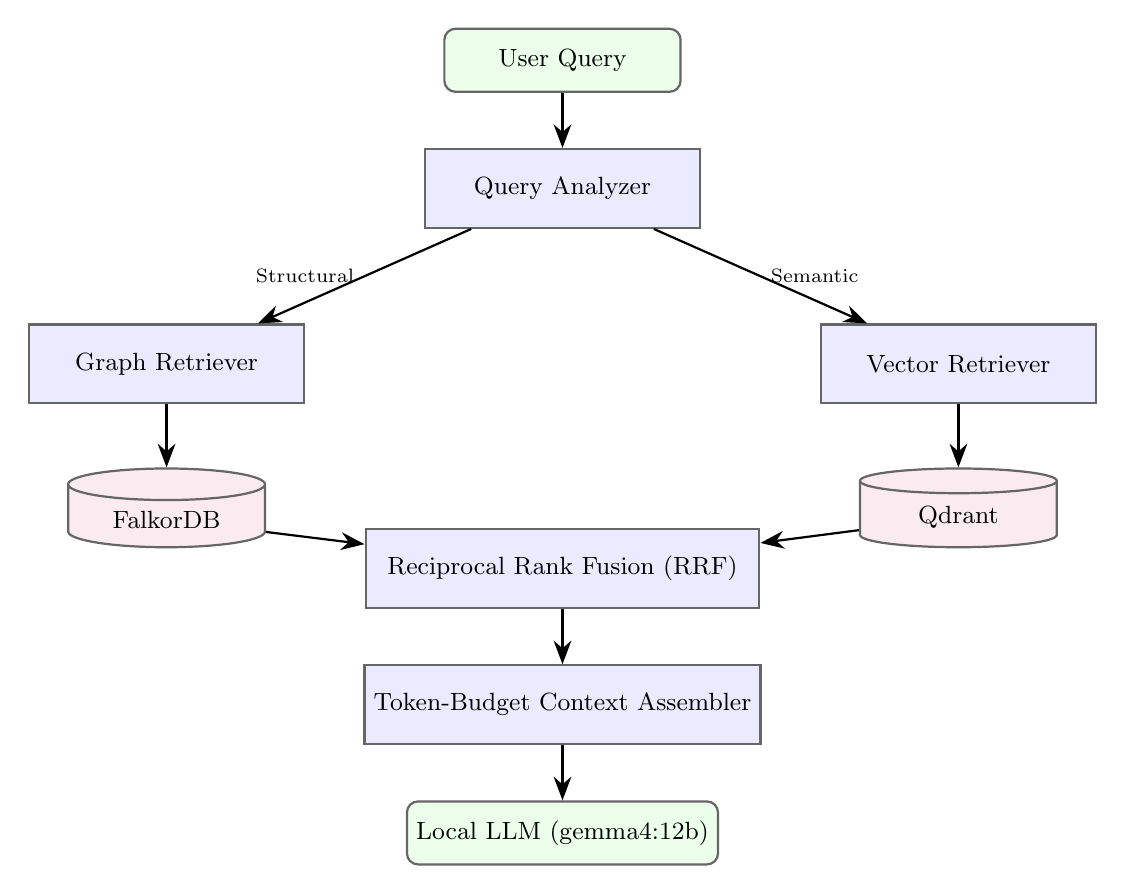
\begin{tikzpicture}[node distance=0.7cm and 1cm, font=\small]
        % Query
        \node[process] (query) {User Query};
        \node[component, below=of query] (analyzer) {Query Analyzer};

        % Parallel paths
        \node[component, below left=1.2cm and 1.5cm of analyzer] (graphret) {Graph Retriever};
        \node[component, below right=1.2cm and 1.5cm of analyzer] (vectorret) {Vector Retriever};

        \node[storage, below=0.8cm of graphret] (fdb2) {FalkorDB};
        \node[storage, below=0.8cm of vectorret] (qdr2) {Qdrant};

        % RRF
        \node[component, below=3.8cm of analyzer, minimum width=5cm] (rrf) {Reciprocal Rank Fusion (RRF)};
        \node[component, below=of rrf, minimum width=5cm] (assembler) {Token-Budget Context Assembler};
        \node[process, below=of assembler] (llm) {Local LLM (gemma4:12b)};

        % Arrows
        \draw[arrow] (query) -- (analyzer);
        \draw[arrow] (analyzer) -- node[left, font=\scriptsize] {Structural} (graphret);
        \draw[arrow] (analyzer) -- node[right, font=\scriptsize] {Semantic} (vectorret);
        \draw[arrow] (graphret) -- (fdb2);
        \draw[arrow] (vectorret) -- (qdr2);
        \draw[arrow] (fdb2) -- (rrf);
        \draw[arrow] (qdr2) -- (rrf);
        \draw[arrow] (rrf) -- (assembler);
        \draw[arrow] (assembler) -- (llm);
    \end{tikzpicture}
    \caption{Concurrent graph--vector path for a generic local query}
    \label{fig:retrieval_flow}
\end{figure}

The figure is not a universal control-flow diagram: global community retrieval and successful exact-relation traversal bypass the parallel fusion branch. This routing avoids paying for or diluting a deterministic graph answer when the query names a supported relation.

\newpage

% ──────────────────────────────────────────────────────────────────────────────
% CHAPTER 3: DETAILED DESIGN
% ──────────────────────────────────────────────────────────────────────────────
\chapter{Detailed Design}

\section{Database Schema}
The system stores parallel data structures in two databases:
\begin{enumerate}
    \item \textbf{Static Relationship Graph (FalkorDB \cite{falkordb2024}):} The graph structure including node labels and relation types is detailed in Table~\ref{tab:graph_schema}.
    \item \textbf{Vector Fragments (Qdrant \cite{qdrant2024}):} Stores 768-dimensional vectors generated from \texttt{nomic-embed-text} alongside a metadata payload including: \texttt{node\_id}, \texttt{file\_path}, \texttt{text\_content}, and \texttt{repository} (used for repository namespace filtering).
\end{enumerate}

\begin{table}[H]
    \centering
    \caption{Implemented FalkorDB node labels and roles}
    \label{tab:graph_schema}
    \small
    \begin{tabular}{p{3.1cm}p{4.5cm}p{5.5cm}}
        \toprule
        \textbf{Node label} & \textbf{Representative properties} & \textbf{Implemented role} \\
        \midrule
        \texttt{RepositoryMetadata} & \texttt{id, repository, last\_indexed\_commit} & Repository identity and synchronization state. \\
        \texttt{Directory} & \texttt{id, name, path, repository} & File-tree hierarchy and module ownership. \\
        \texttt{Module} & \texttt{id, name, file\_path, repository, type} & Python source file and import origin. \\
        \texttt{Class} & \texttt{id, name, file\_path, repository} & Python class definition and inheritance source. \\
        \texttt{Function} & \texttt{id, name, file\_path, signature, repository} & Function or method definition and call source. \\
        \texttt{Document}/\texttt{Configuration} & \texttt{id, name, file\_path, repository, text} & Optional generic Markdown, YAML, and Dockerfile content. \\
        \texttt{Community} & \texttt{id, name, summary, level} & Directory-based architectural summary. \\
        \bottomrule
    \end{tabular}
\end{table}

The implemented relationship vocabulary includes \texttt{DEFINES}, \texttt{IMPORTS}, \texttt{INHERITS}, \texttt{CALLS}, \texttt{USES}, \texttt{DEFINED\_IN}, \texttt{WEAK\_LINK}, \texttt{IN\_COMMUNITY}, and \texttt{COMMUNITY\_DEPENDS}. \texttt{Variable} is reserved as a compatibility target for optional LLM-extracted \texttt{USES} relations; the current AST parser does not emit Variable nodes.

\section{Core Algorithms}
This section examines two implementation mechanisms that materially affect relationship correctness and retrieval ranking:

\subsection{Global Entity Resolution}
\label{sec:entity_resolution}
When a parsed call target cannot be bound immediately, the parser stores an explicit stub such as \texttt{\_\_call\_\_foo}. The resolver uses caller context first and leaves ambiguous targets unresolved instead of creating an arbitrary edge. Figure~\ref{fig:entity_resolution_flow} summarizes the decision order.

\begin{figure}[H]
    \centering
    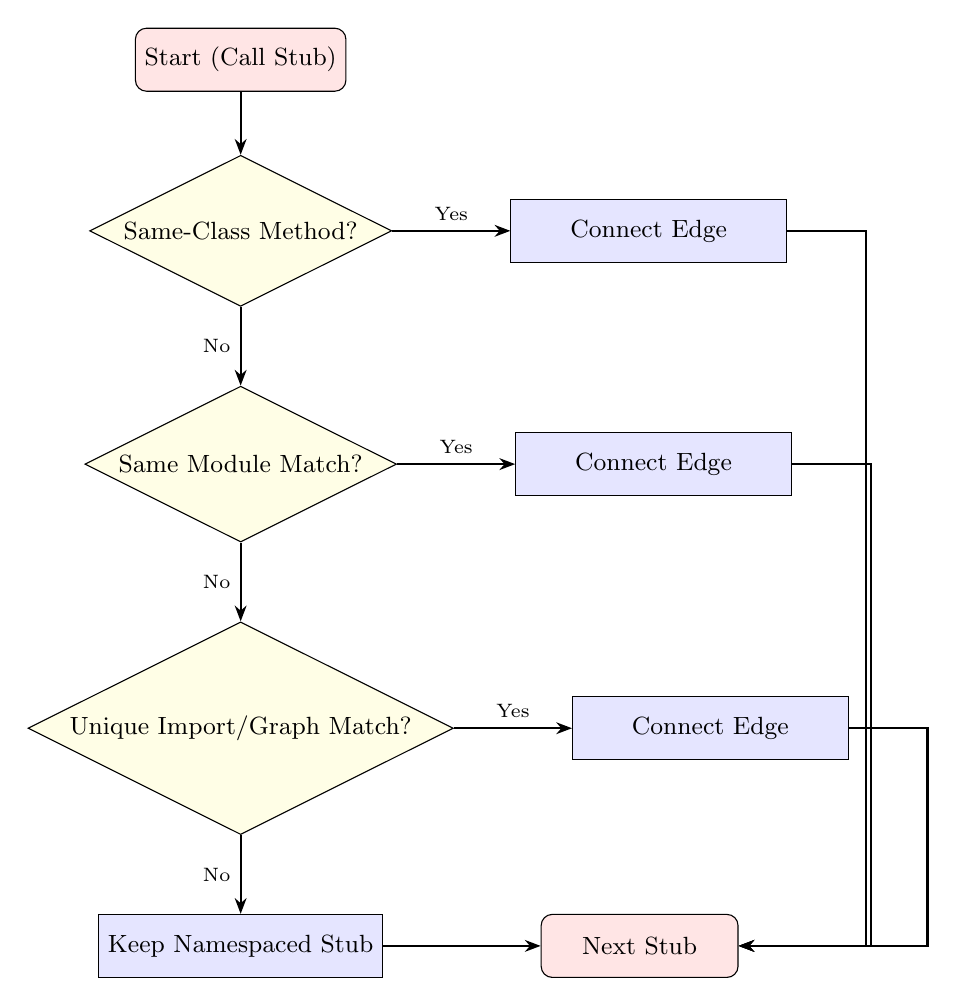
\begin{tikzpicture}[
        node distance=0.8cm and 1cm,
        font=\small,
        startstop/.style={draw, rounded corners, fill=red!10, minimum height=0.8cm, minimum width=2.5cm, text centered},
        process/.style={draw, rectangle, fill=blue!10, minimum height=0.8cm, minimum width=3.5cm, text centered},
        decision/.style={draw, diamond, aspect=2, fill=yellow!10, text centered, inner sep=2pt, minimum width=2.5cm},
        arrow/.style={-{Stealth[length=2mm]}, thick}
    ]
        % Nodes
        \node[startstop] (start) {Start (Call Stub)};
        \node[decision, below=0.8cm of start] (sibling) {Same-Class Method?};
        \node[process, right=1.5cm of sibling] (sibling_ok) {Connect Edge};
        
        \node[decision, below=1cm of sibling] (module) {Same Module Match?};
        \node[process, right=1.5cm of module] (module_ok) {Connect Edge};
        
        \node[decision, below=1cm of module] (global) {Unique Import/Graph Match?};
        \node[process, right=1.5cm of global] (global_ok) {Connect Edge};
        
        \node[process, below=1cm of global] (unresolved) {Keep Namespaced Stub};
        
        \node[startstop, right=2cm of unresolved] (next) {Next Stub};

        % Connections
        \draw[arrow] (start) -- (sibling);
        
        \draw[arrow] (sibling) -- node[above, font=\scriptsize] {Yes} (sibling_ok);
        \draw[arrow] (sibling) -- node[left, font=\scriptsize] {No} (module);
        
        \draw[arrow] (module) -- node[above, font=\scriptsize] {Yes} (module_ok);
        \draw[arrow] (module) -- node[left, font=\scriptsize] {No} (global);
        
        \draw[arrow] (global) -- node[above, font=\scriptsize] {Yes} (global_ok);
        \draw[arrow] (global) -- node[left, font=\scriptsize] {No} (unresolved);
        
        \draw[arrow] (sibling_ok.east) -- ++(1cm,0) |- (next.east);
        \draw[arrow] (module_ok.east) -- ++(1cm,0) |- (next.east);
        \draw[arrow] (global_ok.east) -- ++(1cm,0) |- (next.east);
        \draw[arrow] (unresolved.east) -- (next.west);
    \end{tikzpicture}
    \caption{Decision flow diagram of the Global Entity Resolution process}
    \label{fig:entity_resolution_flow}
\end{figure}

The specific steps in the resolution flow are:
\begin{enumerate}
    \item \textbf{Same-Class Method Check:} For a bare, \texttt{self.}, or \texttt{cls.} call inside a class, the resolver checks for the corresponding method in that same class.
    \item \textbf{Same-Module Function Check:} For an unresolved bare call, the resolver checks for a matching module-level function in the caller's module.
    \item \textbf{Import-Aware and Existing-Graph Check:} The local resolver accepts an imported function only when the import context identifies one candidate. Remaining stubs are queried against previously indexed graph nodes in one batch and are redirected only when exactly one target exists. Ambiguous or missing matches remain explicit and are namespaced by repository.
\end{enumerate}

\subsection{Reciprocal Rank Fusion (RRF)}
When a retrieval path returns one or two ranked lists, the \gls{rrf} algorithm \cite{cormack2009rrf} computes integrated rank scores via:

\begin{equation}
    \text{score}(d) = \sum_{r \in R} \frac{W_r}{k + \text{rank}_r(d)}
    \label{eq:rrf}
\end{equation}

where $k = 60$ is the default smoothing parameter and $W_r$ is the weight for retrieval source $r$. With the checked-in configuration, a successful exact-relation path uses graph-only fusion with configured graph weight 3.0. Generic local fusion caps the graph contribution at 1.0 and uses vector weight 1.0 so noisy neighborhood expansion cannot overpower semantic ranking; vector-only mode uses weights $(0,1)$. The legacy \texttt{hybrid\_weight} setting is retained for compatibility but is not applied by the current retriever. Figure~\ref{fig:rrf_flow} illustrates the two-list accumulation mechanism.

\begin{figure}[H]
    \centering
    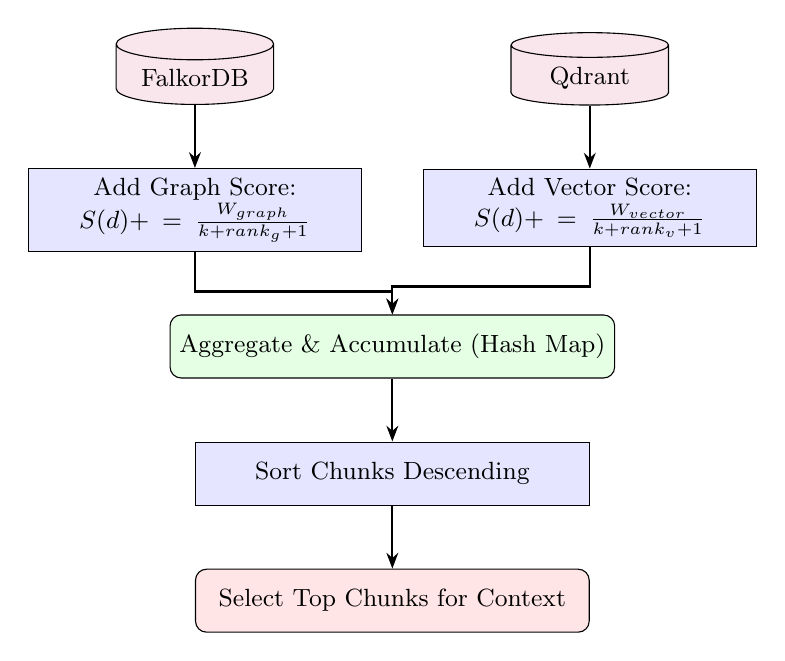
\begin{tikzpicture}[
        node distance=0.8cm and 1cm,
        font=\small,
        databox/.style={draw, cylinder, shape border rotate=90, aspect=0.25, fill=purple!10, minimum height=0.8cm, minimum width=2cm, text centered},
        process/.style={draw, rectangle, fill=blue!10, minimum height=0.8cm, minimum width=4cm, text width=4cm, text centered},
        aggregator/.style={draw, rounded corners, fill=green!10, minimum height=0.8cm, minimum width=5cm, text centered},
        arrow/.style={-{Stealth[length=2mm]}, thick}
    ]
        % Nodes
        \node[databox] (db_graph) {FalkorDB};
        \node[databox, right=3cm of db_graph] (db_vector) {Qdrant};
        
        \node[process, below=0.8cm of db_graph] (score_graph) {Add Graph Score: \\ $S(d) += \frac{W_{graph}}{k + rank_g + 1}$};
        \node[process, below=0.8cm of db_vector] (score_vector) {Add Vector Score: \\ $S(d) += \frac{W_{vector}}{k + rank_v + 1}$};
        
        \node[aggregator, below=3cm of $(db_graph)!0.5!(db_vector)$] (agg) {Aggregate \& Accumulate (Hash Map)};
        \node[process, below=0.8cm of agg, minimum width=5cm] (sort) {Sort Chunks Descending};
        \node[aggregator, below=0.8cm of sort, fill=red!10, minimum width=5cm] (out) {Select Top Chunks for Context};

        % Connections
        \draw[arrow] (db_graph) -- (score_graph);
        \draw[arrow] (db_vector) -- (score_vector);
        \draw[arrow] (score_graph.south) -- ++(0,-0.5cm) -| (agg.north);
        \draw[arrow] (score_vector.south) -- ++(0,-0.5cm) -| (agg.north);
        \draw[arrow] (agg) -- (sort);
        \draw[arrow] (sort) -- (out);
    \end{tikzpicture}
    \caption{Processing flow diagram of the Reciprocal Rank Fusion (RRF) algorithm}
    \label{fig:rrf_flow}
\end{figure}

The steps involved in the RRF scoring flow are:
\begin{enumerate}
    \item \textbf{Initialize Score Map:} Create an empty hash map to store accumulated fusion scores for each candidate document/code chunk.
    \item \textbf{Accumulate Graph Retrieval Scores:} Iterate through FalkorDB query results. For the $i$-th chunk (0-indexed rank), add a score increment of $W_{graph} / (k + i + 1)$ to its map entry.
    \item \textbf{Accumulate Vector Retrieval Scores:} Iterate through Qdrant query results. For the $j$-th chunk, add a score increment of $W_{vector} / (k + j + 1)$ to its map entry.
    \item \textbf{Sort and Filter:} Sort candidate chunks by their accumulated score in descending order, returning the highest-scoring candidates for context assembly.
\end{enumerate}

\section{Community Detection and Architectural Clustering}
\label{sec:community_detection}
A key limitation of low-level graph traversal is that it exposes calls, imports, and inheritance without directly presenting a repository-level architectural summary. The implemented community builder addresses this by grouping entities into repository-scoped directory communities and generating a local summary for each group. API background indexing invokes this step as non-fatal post-processing; the CLI also exposes an explicit \texttt{community-build} command.

\subsection{Directory-Based Partitioning and Summarization}
The final implementation does not use Louvain clustering. An earlier design considered modularity-based communities, but the codebase replaced that approach with deterministic directory partitioning:
\begin{enumerate}
    \item \textbf{Graph projection:} code nodes and typed edges are read from FalkorDB; existing \texttt{Community} nodes are excluded.
    \item \textbf{Repository and directory grouping:} each code node is assigned by the pair \texttt{(repository, dirname(file\_path))}, preventing same-named directories in different repositories from being merged.
    \item \textbf{Local summary generation:} entity lists, internal relations, and boundary relations are serialized and sent to the configured local Ollama model to generate a community title and architectural summary.
    \item \textbf{Persistence:} \texttt{Community}, \texttt{IN\_COMMUNITY}, and weighted \texttt{COMMUNITY\_DEPENDS} relationships are written back to FalkorDB.
\end{enumerate}

\subsection{Integration with the Retrieval Pipeline}
Community nodes serve two purposes:
\begin{itemize}
    \item \textbf{Architectural Navigation:} The interactive visualization portal exposes community nodes as the first drill-down level when a user enters a repository, giving an immediate high-level view of the codebase's logical subsystems.
    \item \textbf{Global-query context:} global retrieval reads repository-filtered community summaries and supplies them to the local answer-generation path.
\end{itemize}

\section{Multi-Repository Knowledge Graph and Visualization Portal}
\label{sec:visualization}
To support engineering workflows involving multiple interdependent codebases (microservices, monorepos, shared libraries), the system implements a \textbf{multi-repository knowledge graph} and a corresponding interactive visualization portal accessible via a web browser.

\subsection{Multi-Repository Master Graph}
A dedicated endpoint (\texttt{GET /graph/master}) constructs a global graph view spanning all indexed repositories:
\begin{itemize}
    \item Each repository is represented by a \texttt{RepositoryMetadata} node.
    \item \texttt{Directory} nodes are automatically generated from parsed source file paths --- including repositories that consist entirely of Python code files, ensuring structural coverage regardless of the presence of non-code files (\texttt{.yaml}, \texttt{.md}).
    \item Noise directories (\texttt{node\_modules}, \texttt{.venv}, \texttt{.agents}, \texttt{\_\_pycache\_\_}, \texttt{.git}, etc.) are filtered at the Cypher query level, preventing stale legacy nodes from polluting the master graph.
\end{itemize}

\subsection{Hierarchical Drill-Down Navigation}
The portal implements a three-level navigation hierarchy, illustrated in Figure~\ref{fig:navigation_hierarchy}:

\begin{figure}[H]
    \centering
    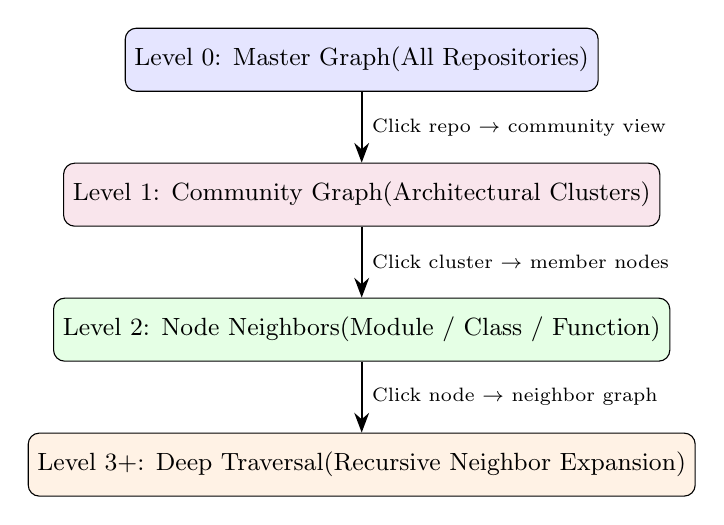
\begin{tikzpicture}[
        node distance=0.9cm and 1.2cm,
        font=\small,
        level/.style={draw, rounded corners, fill=blue!10, minimum height=0.8cm, minimum width=3.8cm, text centered},
        level2/.style={draw, rounded corners, fill=purple!10, minimum height=0.8cm, minimum width=3.8cm, text centered},
        level3/.style={draw, rounded corners, fill=green!10, minimum height=0.8cm, minimum width=3.8cm, text centered},
        level4/.style={draw, rounded corners, fill=orange!10, minimum height=0.8cm, minimum width=3.8cm, text centered},
        arrow/.style={-{Stealth[length=2.5mm]}, thick}
    ]
        \node[level] (master) {Level 0: Master Graph\\ (All Repositories)};
        \node[level2, below=of master] (community) {Level 1: Community Graph\\ (Architectural Clusters)};
        \node[level3, below=of community] (node) {Level 2: Node Neighbors\\ (Module / Class / Function)};
        \node[level4, below=of node] (deep) {Level 3+: Deep Traversal\\ (Recursive Neighbor Expansion)};

        \draw[arrow] (master) -- node[right, font=\scriptsize] {Click repo $\rightarrow$ community view} (community);
        \draw[arrow] (community) -- node[right, font=\scriptsize] {Click cluster $\rightarrow$ member nodes} (node);
        \draw[arrow] (node) -- node[right, font=\scriptsize] {Click node $\rightarrow$ neighbor graph} (deep);
    \end{tikzpicture}
    \caption{Hierarchical navigation model of the multi-repository graph portal}
    \label{fig:navigation_hierarchy}
\end{figure}

A \textbf{breadcrumb navigation bar} persists across all levels, rendering the complete drill-down path (e.g., \texttt{Master $\triangleright$ langchain-core $\triangleright$ Retrieval Cluster $\triangleright$ BaseRetriever}). Any intermediate node in the breadcrumb is clickable, allowing the user to jump back to any previously visited level without losing context.

\subsection{Performance Optimizations for Concurrent Indexing}
Two bounded-concurrency mechanisms are implemented:
\begin{itemize}
    \item \textbf{Concurrent repository indexing:} API background jobs use an \texttt{asyncio.Semaphore} whose \texttt{INDEXING\_CONCURRENCY} default is 3.
    \item \textbf{Parallel AST parsing:} files within one repository are parsed with a bounded \texttt{ThreadPoolExecutor}; the worker limit is derived from CPU count and capped at 32.
\end{itemize}
These mechanisms are present and unit-tested, but the thesis does not claim an end-to-end indexing speedup because no controlled sequential-versus-concurrent repository benchmark is persisted.

\section{Programming-Language Scalability}
The storage ports, repository namespaces, rank fusion, and context assembly are largely language-independent after canonical entities and chunks exist. The ingestion semantics are not. The production indexing boundary currently accepts only \texttt{languages=["python"]}; Java-only repositories are rejected, and the parser returns an explicit not-implemented error for Java extraction. Supporting another language requires a Tree-Sitter grammar, language-specific entity and relation extraction, canonical symbol resolution, chunk construction, and language-specific ground-truth tests. The existing Java-aware skeletonizer only formats already selected Java files and does not constitute Java indexing support. Kubernetes, whose principal implementation language is Go, therefore cannot be used as a comparable AST benchmark until a Go ingestion adapter is implemented.

\section{Software Testing}
The codebase is validated via 313 passing automated tests, with 27 explicitly skipped integration cases and two warnings in the final merged verification. The suite covers parsing and extraction logic, end-to-end ingestion pipelines, evaluation preflight, and functional API surfaces. The answer-quality benchmark itself is a separate 180-run controlled workload and is not counted as unit-test coverage.

\newpage

% ──────────────────────────────────────────────────────────────────────────────
% CHAPTER 4: EXPERIMENTAL RESULTS AND DISCUSSION
% ──────────────────────────────────────────────────────────────────────────────
\chapter{Experimental Results and Discussion}

\section{Test Environment}
\begin{itemize}
    \item \textbf{Hardware:} Apple Mac mini M4 developer machine; the benchmark records local execution but does not claim a hardware-independent latency.
    \item \textbf{Software:} Python 3.12, FalkorDB, Qdrant, and Ollama with local embedding and generation endpoints.
    \item \textbf{Indexed source:} Pinned \texttt{llama-index-core==0.14.21}; deterministic source digest \texttt{sha256:13b55bcf111885b7c2c9c07886b5656769041331c81c28bcf3cbfb87939ec509}; schema version 3; embedding model \texttt{nomic-embed-text}.
    \item \textbf{Answer-quality suite:} 30 cases (10 simple, 10 medium, 10 hard), two retrieval modes, three repeats, seed 42, for 180 generated and scored answers.
    \item \textbf{Statistical unit:} the 30 question cases; the three repeats are averaged within each case before paired bootstrap resampling.
\end{itemize}

\section{Metrics Justification}
\label{sec:metrics_justification}
We selected evaluation metrics based on: (i) suitability to the code retrieval task, and (ii) comparability with prior research.

\begin{itemize}
    \item \textbf{Hit Rate @K} (K=5): Measures the frequency of relevant documents appearing in the top-K returned results. Selected over Precision@K because in developer assistance, the user needs *at least one correct code block* to proceed, rather than all K blocks being correct \cite{thakur2021beir}.
    \item \textbf{Faithfulness} (RAGAS \cite{shahul2023ragas}): Evaluates how loyal the generated answer is to the retrieved context, revealing LLM hallucinations.
    \item \textbf{Answer Relevancy} (RAGAS \cite{shahul2023ragas}): Measures how relevant the generated answer is to the user's question, complementary to Faithfulness.
    \item \textbf{Answer Correctness} (RAGAS \cite{shahul2023ragas}): Compares the generated answer with the reviewed reference answer.
    \item \textbf{Paired 95\% Confidence Interval}: Quantifies uncertainty in Hybrid-minus-vector differences by resampling the 30 question-level pairs with replacement. Repeats are averaged within a case to avoid treating them as independent questions.
    \item \textbf{Latency Breakdown}: Segmenting processing time by phase helps target bottlenecks.
\end{itemize}

BLEU and ROUGE were not selected as confirmatory metrics because lexical overlap does not directly test whether an answer is grounded in retrieved evidence or correct about code relationships.

\section{Evidence Provenance and Excluded Historical Diagnostic}
The repository also contains a historical 50-case structural report generated against a schema-v2 index. Its current status file explicitly records that it predates the schema-v3 identity repair and that its RAGAS field is null. Because it does not satisfy the present provenance preflight, this thesis does not use its Hit Rate values as current confirmatory evidence. The analysis below is therefore restricted to the completed schema-v3 answer-quality artifact, whose source digest, index run, embedding model, raw records, and review grade are persisted.

\section{Independent Answer-Quality Benchmark}
We separately measured generated-answer quality with the RAGAS metrics \cite{shahul2023ragas}. The workload contains 30 source-reviewed cases (10 simple, 10 medium, and 10 hard), evaluates vector-only and Hybrid-RAG modes, and repeats each case three times with seed 42. The answer model is local \texttt{gemma4:12b}; an independent local \texttt{qwen2.5-coder:7b} judge scores Faithfulness, Answer Relevancy, and Answer Correctness. The complete workload contains 180 generated and scored records.

\begin{table}[H]
    \centering
    \caption{Answer quality with paired case-level 95\% confidence intervals}
    \label{tab:answer_quality_results}
    \resizebox{\textwidth}{!}{%
    \begin{tabular}{lccc}
        \toprule
        \textbf{Metric} & \textbf{Vector mean [95\% CI]} & \textbf{Hybrid mean [95\% CI]} & \textbf{$\Delta$ [95\% CI]} \\
        \midrule
        Faithfulness & 0.896 [0.816, 0.956] & 0.924 [0.843, 0.980] & +0.029 [$-0.069$, 0.115] \\
        Answer Relevancy & 0.729 [0.618, 0.826] & 0.808 [0.737, 0.859] & +0.079 [$-0.0001$, 0.175] \\
        Answer Correctness & 0.652 [0.606, 0.703] & 0.698 [0.650, 0.748] & +0.046 [0.002, 0.094] \\
        \bottomrule
    \end{tabular}
    }
\end{table}

The point estimates favor Hybrid-RAG for all three metrics, but the paired intervals change the strength of the conclusion. Faithfulness includes both negative and positive differences. Answer Relevancy is borderline and still touches zero at the reported precision. Only Answer Correctness has a 95\% interval entirely above zero. This is evidence uncertainty, not proof of a software defect. All 180 records received valid scores and all had a source hit. The gold answers were approved by an AI source review, not independent human annotation; therefore the result is controlled local evidence rather than a human-evaluated production accuracy rate.

\section{Generalizability and Baseline Coverage}
The instructor's requested multi-repository evaluation is not yet complete. Table~\ref{tab:evaluation_coverage} separates completed evidence from planned experiments.

\begin{table}[H]
    \centering
    \caption{Repository and baseline coverage}
    \label{tab:evaluation_coverage}
    \begin{tabular}{p{3.2cm}p{3.2cm}p{6.4cm}}
        \toprule
        \textbf{Target} & \textbf{Status} & \textbf{Interpretation} \\
        \midrule
        LlamaIndex Core & Completed & 30 reviewed questions, 3 repeats, Hybrid and vector-only modes. \\
        Transformers & Not executed & Requires a pinned source artifact and reviewed repository-specific questions. \\
        LangChain & Not executed & Requires an independent index, source digest, and gold dataset. \\
        Kubernetes & Not comparable yet & Primarily Go; the current AST ingestion pipeline is Python-only. \\
        BM25 / graph-only / GraphRAG & Not executed & Required to distinguish hybrid gains from lexical, graph-only, and alternative graph-RAG designs. \\
        \bottomrule
    \end{tabular}
\end{table}

Consequently, the benchmark answers RQ1--RQ3 only for the pinned LlamaIndex workload. It does not establish generalization across repositories, programming languages, or retrieval families.

\section{Architectural Optimization and Enhancements}
The implemented reliability improvements are evaluated as engineering controls rather than collapsed into one unsupported optimization percentage. When a repository is supplied as query scope, repository filtering prevents results from other namespaces; without that optional scope, retrieval may search across indexed repositories. Index replacement writes the new graph and vector records before stale data is removed, reducing an empty-index window, but it does not provide reader-isolated generation cutover. Provenance checks require matching source identity, index run, schema, and embedding model; cache generations separate responses after indexing; and unsupported Java input is rejected before indexing. Optional YAML, Markdown, and Dockerfile ingestion is generic document/configuration chunking and is disabled by default; it does not provide Python-style AST semantics.

These controls make the retrieval and evaluation measurements reproducible. They should not be described as a single token-savings or accuracy percentage without a separate controlled experiment.

\section{Latency Breakdown}
The completed answer-quality benchmark recorded retrieval, local generation, and token statistics for both retrieval modes. Table~\ref{tab:latency_breakdown} reports case-level means and paired-bootstrap intervals; these are not service-level percentiles.

\begin{table}[H]
    \centering
    \caption{Latency breakdown of system processes}
    \label{tab:latency_breakdown}
    \resizebox{\textwidth}{!}{%
    \begin{tabular}{lccc}
        \toprule
        \textbf{Measure} & \textbf{Vector mean [95\% CI]} & \textbf{Hybrid mean [95\% CI]} & \textbf{$\Delta$ [95\% CI]} \\
        \midrule
        Retrieval latency (ms) & 134 [118, 151] & 371 [348, 395] & +237 [208, 266] \\
        Generation latency (ms) & 96,754 [84,413, 110,142] & 87,268 [78,110, 96,465] & $-9,486$ [$-23,036$, 1,438] \\
        Prompt tokens & 1,841 [1,633, 2,047] & 1,740 [1,566, 1,913] & $-101$ [$-282$, 77] \\
        Completion tokens & 934 [788, 1,092] & 834 [734, 938] & $-100$ [$-259$, 30] \\
        \bottomrule
    \end{tabular}
    }
\end{table}

Hybrid retrieval adds a measured 237 ms of retrieval time, with a paired 95\% interval of 208--266 ms, in this workload. The intervals for generation latency and token deltas include zero, so their apparent reductions are not conclusive. Local generation dominates end-to-end latency for both modes; the result supports a sub-second mean retrieval claim on this machine, not a sub-second answer-response SLA.

\section{Case Study}
To illustrate practical feasibility, we trace the benchmark query: ``\textit{What sequence does BaseRetriever.retrieve follow when it receives a plain query string, including callbacks and recursive retrieval?}''.

\begin{enumerate}
    \item \textbf{Question analysis:} The query names \texttt{BaseRetriever.retrieve} and asks for an execution sequence involving callbacks and recursive retrieval.
    \item \textbf{Retrieval channels:}
    \begin{itemize}
        \item FalkorDB contributes structural relationships around the retriever implementation.
        \item Qdrant retrieves semantically similar chunks from \texttt{base/base\_retriever.py} and \texttt{retrievers/recursive\_retriever.py}.
    \end{itemize}
    \item \textbf{RRF Rank Fusion:} The graph and vector ranked lists are fused before context assembly.
    \item \textbf{Benchmark context selection:} The benchmark keeps the first five fused results and formats them directly as contexts. This case does not exercise the API's optional dynamic token-budget parameters.
    \item \textbf{Generation:} The answer explains the callback start, query-bundle conversion, retrieval, recursive resolution, callback completion, and return sequence. One case illustrates the path; aggregate quality is reported in Table~\ref{tab:answer_quality_results}.
\end{enumerate}

\newpage

% ──────────────────────────────────────────────────────────────────────────────
% CHAPTER 5: CONCLUSION & FUTURE WORK
% ──────────────────────────────────────────────────────────────────────────────
\chapter{Conclusion and Future Work}

\section{Conclusion}
The completed experiment supports a narrower conclusion than the earlier point-estimate-only report:
\begin{enumerate}
    \item \textbf{RQ1:} Hybrid-RAG has higher point estimates for Faithfulness (+0.029), Answer Relevancy (+0.079), and Answer Correctness (+0.046) on the pinned LlamaIndex workload.
    \item \textbf{RQ2:} Mean retrieval latency increases from 134 ms to 371 ms. Local generation remains dominant at approximately 87--97 seconds; observed token and generation-latency reductions have intervals that include zero.
    \item \textbf{RQ3:} Only the Answer Correctness difference has a paired 95\% confidence interval entirely above zero. Faithfulness is inconclusive, and Answer Relevancy is borderline at zero. These results do not establish cross-repository or cross-language superiority.
\end{enumerate}

The principal technical contributions are:
\begin{itemize}
    \item query-aware graph and vector retrieval with deterministic relation plans, weighted rank fusion, sibling expansion, and budgeted context assembly;
    \item repository identity scoping when supplied, replacement-before-delete indexing, provenance, cache-generation, and local-provider controls that make retrieval and evaluation runs auditable;
    \item deterministic directory-based communities with local Ollama-generated summaries, persisted dependencies, and repository-filtered global retrieval;
    \item a multi-repository 3D/2D visualization portal and bounded-concurrency indexing implementation; and
    \item a reproducible 180-record benchmark plus a deterministic paired case-level confidence-interval analysis.
\end{itemize}

\section{Limitations}
\label{sec:limitations}
\begin{itemize}
    \item \textbf{Local Generation Latency:} Answer generation averages approximately 87 seconds for hybrid retrieval and 97 seconds for vector-only retrieval on the measured developer machine; this is not a sub-second end-to-end system.
    \item \textbf{Language Constraints:} Semantic AST indexing currently supports Python only. Java projects are rejected explicitly, and optional non-code ingestion provides generic chunks rather than language-aware AST semantics.
    \item \textbf{Evaluation Scale:} The complete answer-quality benchmark uses one pinned Python repository and AI-reviewed reference answers. Confidence intervals quantify within-workload uncertainty, but additional repositories and independent human review are still required for generalization.
    \item \textbf{Baseline Coverage:} Only vector-only retrieval is executed under the paired protocol. BM25, graph-only retrieval, learned code encoders, and an independent GraphRAG implementation are not measured.
    \item \textbf{Cost Evidence:} Local Ollama produces no hosted API bill in this experiment, but the benchmark does not measure electricity, hardware depreciation, storage, or maintenance cost.
    \item \textbf{Statistical Power:} Faithfulness and Answer Relevancy intervals include or touch zero. More independent questions are required before interpreting their positive point estimates as reliable improvements.
\end{itemize}

\section{Future Work}
\begin{itemize}
    \item \textbf{Multi-Repository Replication:} Build independent, source-reviewed workloads for at least Transformers and LangChain, pin each source identity, and report per-repository and pooled paired intervals.
    \item \textbf{Additional Baselines and Ablations:} Execute BM25, graph-only, vector-only, Hybrid-RAG, and a documented external GraphRAG baseline under matched questions and generation settings.
    \item \textbf{Language Adapters:} Add complete entity extraction, relation resolution, chunking, and tests for Java and Go before using Java projects or Kubernetes as evaluation corpora.
    \item \textbf{Ambiguous Cross-Repository Resolution:} Extend the current unique-match resolver with import-aware namespace disambiguation, then evaluate cross-repository relation questions explicitly.
    \item \textbf{Human Review and Power Analysis:} Add independent human reference review and determine the number of cases required to narrow the confidence intervals for each quality metric.
    \item \textbf{Adaptive RRF Weights:} Tune graph and vector weights on a separate development set and evaluate them on untouched repositories to avoid test-set optimization.
\end{itemize}

% ──────────────────────────────────────────────────────────────────────────────
% BIBLIOGRAPHY
% ──────────────────────────────────────────────────────────────────────────────
\begin{thebibliography}{99}

\bibitem{lewis2020rag}
P.~Lewis, E.~Perez, A.~Piktus, F.~Petroni, V.~Karpukhin, N.~Goyal, H.~K{\"u}ttler, M.~Lewis, W.-T.~Yih, T.~Rockt{\"a}schel, S.~Riedel, and D.~Kiela, ``Retrieval-augmented generation for knowledge-intensive NLP tasks,'' in \textit{Advances in Neural Information Processing Systems (NeurIPS)}, vol.~33, pp. 9459--9474, 2020.

\bibitem{cormack2009rrf}
G.~V.~Cormack, C.~L.~A.~Clarke, and S.~B{\"u}ttcher, ``Reciprocal rank fusion outperforms condorcet and individual rank learning methods,'' in \textit{Proceedings of the 32nd International ACM SIGIR Conference on Research and Development in Information Retrieval}, pp. 758--759, 2009.

\bibitem{bm25}
S.~Robertson and H.~Zaragoza, ``The probabilistic relevance framework: BM25 and beyond,'' \textit{Foundations and Trends in Information Retrieval}, vol.~3, no.~4, pp. 333--389, 2009.

\bibitem{edge2024graphrag}
D.~Edge, H.~Trinh, N.~Cheng, J.~Bradley, A.~Chao, C.~Mody, S.~Truitt, and J.~Larson, ``From local to global: A graph RAG approach to query-focused summarization,'' \textit{arXiv preprint arXiv:2404.16130}, 2024.

\bibitem{treesitter}
M.~Brunsfeld, ``Tree-sitter: An incremental parsing system for programming tools,'' GitHub, 2018. [Online]. Available: \url{https://tree-sitter.github.io/tree-sitter/}

\bibitem{liu2023lost}
N.~F.~Liu, K.~Lin, J.~Hewitt, A.~Paranjape, M.~Bevilacqua, F.~Petroni, and P.~Liang, ``Lost in the middle: How language models use long contexts,'' \textit{Transactions of the Association for Computational Linguistics}, vol.~12, pp. 157--173, 2024.

\bibitem{shahul2023ragas}
S.~Es, J.~James, L.~Espinosa-Anke, and S.~Schockaert, ``RAGAS: Automated evaluation of retrieval augmented generation,'' in \textit{Proceedings of the 18th Conference of the European Chapter of the Association for Computational Linguistics: System Demonstrations}, pp. 150--163, 2024.

\bibitem{chen2021codex}
M.~Chen, J.~Tworek, H.~Jun, Q.~Yuan, H.~Pinto de Oliveira, J.~Kaplan, H.~Edwards, Y.~Burda, N.~Joseph, G.~Brockman, \textit{et al.}, ``Evaluating large language models trained on code,'' \textit{arXiv preprint arXiv:2107.03374}, 2021.

\bibitem{feng2020codebert}
Z.~Feng, D.~Guo, D.~Tang, N.~Duan, X.~Feng, M.~Gong, L.~Shou, B.~Qin, T.~Liu, D.~Jiang, and M.~Zhou, ``CodeBERT: A pre-trained model for programming and natural languages,'' in \textit{Findings of the Association for Computational Linguistics: EMNLP 2020}, pp. 1536--1547, 2020.

\bibitem{li2023starcoder}
R.~Li, L.~B.~Allal, Y.~Zi, N.~Muennighoff, D.~Kocetkov, C.~Mou, M.~Marone, C.~Akiki, J.~Li, J.~Chim, \textit{et al.}, ``StarCoder: May the source be with you!,'' \textit{Transactions on Machine Learning Research}, 2023.

\bibitem{deepseek2024coder}
D.~Guo, Q.~Zhu, D.~Yang, Z.~Xie, K.~Dong, W.~Zhang, G.~Chen, X.~Bi, Y.~Wu, Y.~K.~Li, \textit{et al.}, ``DeepSeek-Coder: When the large language model meets programming --- the rise of code intelligence,'' \textit{arXiv preprint arXiv:2401.14196}, 2024.

\bibitem{copilot2022}
S.~Kalliamvakou, ``Research: Quantifying GitHub Copilot's impact on developer productivity and happiness,'' GitHub Blog, 2022. [Online]. Available: \url{https://github.blog/news-insights/research/research-quantifying-github-copilots-impact-on-developer-productivity-and-happiness/}

\bibitem{guo2024graphcodebert}
D.~Guo, S.~Ren, S.~Lu, Z.~Feng, D.~Tang, S.~Liu, L.~Zhou, N.~Duan, A.~Svyatkovskiy, S.~Fu, \textit{et al.}, ``GraphCodeBERT: Pre-training code representations with data flow,'' in \textit{International Conference on Learning Representations (ICLR)}, 2021.

\bibitem{cockburn2005hexagonal}
A.~Cockburn, ``Hexagonal architecture,'' 2005. [Online]. Available: \url{https://alistair.cockburn.us/hexagonal-architecture/}

\bibitem{falkordb2024}
FalkorDB Contributors, ``FalkorDB: Ultra-fast graph database,'' 2024. [Online]. Available: \url{https://www.falkordb.com/}

\bibitem{qdrant2024}
Qdrant Team, ``Qdrant: Vector similarity search engine,'' 2024. [Online]. Available: \url{https://qdrant.tech/}

\bibitem{nussbaum2024nomic}
Z.~Nussbaum, J.~Morris, B.~Duderstadt, and A.~Mulyar, ``Nomic Embed: Training a reproducible long context text embedder,'' \textit{arXiv preprint arXiv:2402.01613}, 2024.

\bibitem{ollama2024}
Ollama Contributors, ``Ollama: Run large language models locally,'' 2024. [Online]. Available: \url{https://ollama.com/}

\bibitem{llamaindex2024}
J.~Liu, ``LlamaIndex: Data framework for LLM applications,'' 2024. [Online]. Available: \url{https://www.llamaindex.ai/}

\bibitem{xia2023devtime}
C.~S.~Xia, Y.~Deng, S.~Dunn, and L.~Zhang, ``Automated program repair in the era of large pre-trained language models,'' in \textit{Proceedings of the 45th International Conference on Software Engineering (ICSE)}, pp. 1482--1494, 2023.

\bibitem{thakur2021beir}
N.~Thakur, N.~Reimers, A.~R{\"u}ckl{\'e}, A.~Srivastava, and I.~Gurevych, ``BEIR: A heterogeneous benchmark for zero-shot evaluation of information retrieval models,'' in \textit{Proceedings of the 35th Conference on Neural Information Processing Systems (NeurIPS)}, 2021.

\end{thebibliography}

\end{document}
